\documentclass{article}
\usepackage{tikz}
\usetikzlibrary{positioning, fit, shapes}
\pagenumbering{gobble}
\begin{document}
\begin{figure}
\centering
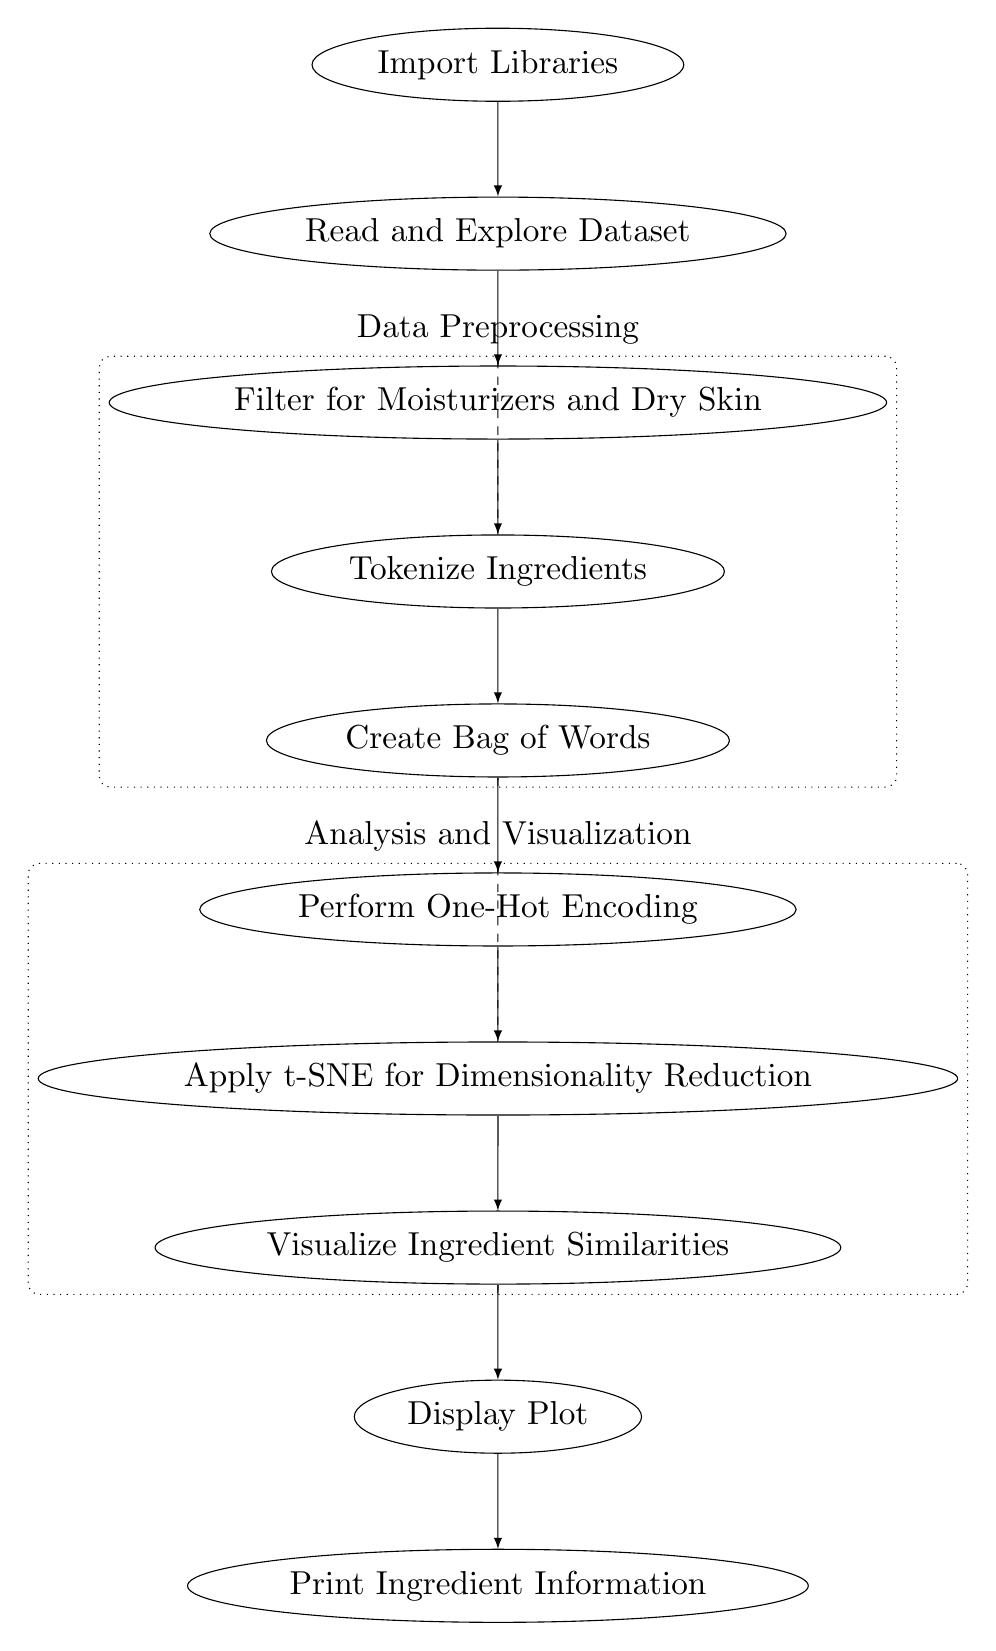
\begin{tikzpicture}[scale=1.2, transform shape]

% Use case nodes
\node[ellipse, draw] (import) {Import Libraries};
\node[ellipse, draw, below=1cm of import] (read) {Read and Explore Dataset};
\node[ellipse, draw, below=1cm of read] (filter) {Filter for Moisturizers and Dry Skin};
\node[ellipse, draw, below=1cm of filter] (tokenize) {Tokenize Ingredients};
\node[ellipse, draw, below=1cm of tokenize] (bagofwords) {Create Bag of Words};
\node[ellipse, draw, below=1cm of bagofwords] (onehot) {Perform One-Hot Encoding};
\node[ellipse, draw, below=1cm of onehot] (tsne) {Apply t-SNE for Dimensionality Reduction};
\node[ellipse, draw, below=1cm of tsne] (visualize) {Visualize Ingredient Similarities};
\node[ellipse, draw, below=1cm of visualize] (display) {Display Plot};
\node[ellipse, draw, below=1cm of display] (print) {Print Ingredient Information};

% Use case connections
\draw[-latex] (import) -- (read);
\draw[-latex] (read) -- (filter);
\draw[-latex] (filter) -- (tokenize);
\draw[-latex] (tokenize) -- (bagofwords);
\draw[-latex] (bagofwords) -- (onehot);
\draw[-latex] (onehot) -- (tsne);
\draw[-latex] (tsne) -- (visualize);
\draw[-latex] (visualize) -- (display);
\draw[-latex] (display) -- (print);

% Fit node
\node[draw, dotted, rounded corners, fit=(filter) (tokenize) (bagofwords), label=above:Data Preprocessing] (data) {};
\node[draw, dotted, rounded corners, fit=(onehot) (tsne) (visualize), label=above:Analysis and Visualization] (analysis) {};

% Relationships
\draw[dashed] (filter) -- (data);
\draw[dashed] (tokenize) -- (data);
\draw[dashed] (bagofwords) -- (data);
\draw[dashed] (onehot) -- (analysis);
\draw[dashed] (tsne) -- (analysis);
\draw[dashed] (visualize) -- (analysis);

\end{tikzpicture}
\caption{Use Case Diagram: Project Flow}
\end{figure}
\end{document}
